\chapter{Time Discrimination-TDC}\label{ch:TDC}
% walk error - amplitude, compare with analytical results
% compare look up table between real and simulate relation
% results w/o fitlers and results after filter
% error for different methods
In this section, the TDC modeling will be introduced first followed by the application of different timing algorithms to simulated return signals from different target distances. The slew-rate compensation is not included due to the usage of two thresholds. The two-threshold configuration makes weak return signal invisible to the system because when the amplitude of the return pulse is lower than the higher threshold, the comparator will not be triggered, and the algorithm will ignore the pulse. In addition, the time-variant thresholding is not included in this section either since the R and C values of the photon detector are not available in this study, which makes it difficult to calibrate the parameter A and B in Equation \eqref{eq:TDC_time1}, and therefore, modeling the time-variant thresholding is impractical.
% TDC modeling
\section{TDC Modeling}
%{Propagation delay}
\subsection{Propagation delay}
As shown in Figure \ref{fig:TDC_schematic}, the comparator is one of the key components of the TDC. In practice, a TDC circuit requires a small amount of time to respond and propagate signals for voltage comparison, so the comparators have a propagation delay, which limits the fastest frequency of a signal the TDC can process [4]. However, on the other hand, even though the propagation delay restrains the frequency of the signal to be processed, slower fluctuation still exists in the transient signal inside the comparator, caused by the unstable transient response of the electrical device to high-frequency oscillation. To model the response of the TDC to the input analog signal, we have to simulate the transient signal, but the transient response of an electrical device to a rapid oscillating signal is usually ill-defined, which makes the modeling difficult. In this study, inspired by Wahab [1], we approximated the transient signal by sub-sampling the original ‘continuous' signal with a sampling rate of 2GHz and smoothing the sub-sampled signal by a spline-line fitting, assuming no additional high-frequency noises were added to the transient signals before comparison. One should note that the approximation is one of the simplified versions of the transient signal. In a real device, the transient signal may not follow the same behavior as described above. Moreover, the sub-sampling rate (2 GHz) was obtained from the bandwidth of a high-speed comparator defined by its propagation delay $\tau_{delay}$ (0.25 ns): $bandwidth = 1/2\tau_{delay}$ [2]. An example of the signal after subsampling is shown in Figure \ref{fig:TDC_subsampling}.
% If a signal was sampled at a frequency lower than 2 GHz, no sub-sampling was performed before the spline-line fitting because the bandwidth of the signal is already smaller than the bandwidth of the comparator.
\begin{figure}[t!p]
\centering
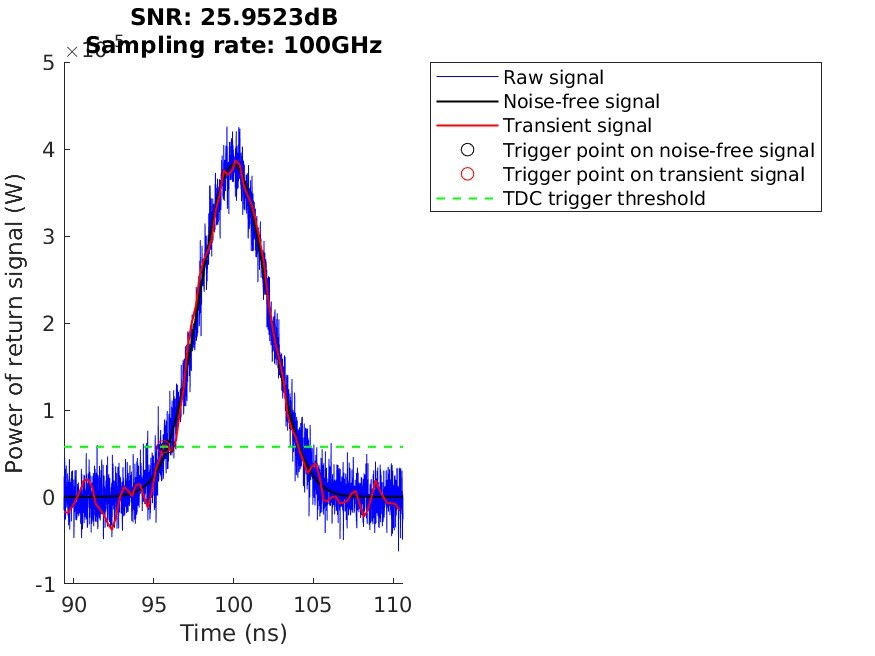
\includegraphics[width=.8\textwidth]{figures/chapter7_TDC/fig_subsampling.jpg}
\caption{The ‘continuous’ return signal after subsampling}
\label{fig:TDC_subsampling}
\end{figure}
% Linear Interpolation
\subsection{Linear interpolation}
The sampling rate of the signal is set to 100GHz or 10ps, and the TDC resolution was set to 1 ps [3]. The resolution was achieved in the TDC model by linearly interpolating the transient signals to a grid of 1 ps, and whenever a point on the grid excessed the threshold, the corresponding time was measured as the arrival time. The linear interpolation is applied to the trigger events of all the TDC-based timing algorithms. An example of the interpolation for the traditional leading-edge algorithm is shown in Figure \ref{fig:TDCinterpolation}.
\begin{figure}[t!p]
\centering
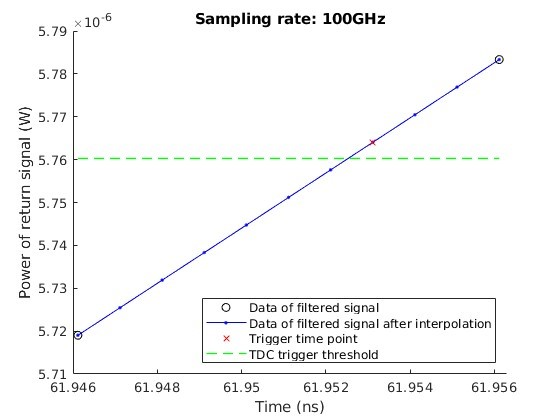
\includegraphics[width=.8\textwidth]{figures/chapter7_TDC/TDC_interpolation.jpg}
\caption{Illustration of interpolation for leading-edge detection }
\label{fig:TDCinterpolation}
\end{figure}
% threshold
\subsection{TDC trigger threshold}
The setting of the trigger threshold of a TDC is also important because too low or too high threshold will increase the false triggering by the noise (PFA) or decrease the sensitivity of the algorithm to weak return signals (PD). To balance the trade-off between PFA and PD, in this study we determine the threshold by the probability of false positive. Here we assume the noise of the electrical system is Gaussian distributed white noise. Theoretically, the threshold can be determined by:
\begin{align} \label{eq:TDC_threshold}
    V_{th}=\sigma_0Q^{-1}\left(P_{fa}\right)+\mu_0
\end{align}
where $\mu_0$ is the mean of the noise which is equal to zero, $\sigma_0$ is the STD of the noise of the signal with laser off, and Q is the complementary cumulative distribution function (CCDF) of the Gaussian white noise, defined by
\begin{align}
    Q\left(x\right)=\frac{1}{2}efc\left(\frac{x}{\sqrt2}\right)
\end{align}
% experiement
\section{Experiment and Timing algorithms}
\subsection{Experimental design}
Monte-Carlo experiment was conducted using 500 observations of transmit and return signals. The target distance ranges from 5 to 60m with an increment of 2.5m. The return signals were generated by the pulse model, the propagation model, and the noise model. The key parameters used in those models are given below with other parameters unchanged.
\begin{table}
\caption{{Parameters in lidar models}}
\centering
\label{table:lidarspec}
\begin{tabular}{|l|l|l|}
\hline
Parameters    & Values \\ \hline
Peak power & $300 W$              \\ \hline
Sampling rate & $100~GHz$      \\ \hline
Target reflectivity & $10\%$     \\ \hline
BW due to comparator propagation delay & $2~GHz$        \\ \hline
\end{tabular}%
\end{table}
% threshold
\subsection{TDC trigger threshold}
The PFA is preset to 0.001 in this study, and it was evaluated on 100 observations of noise signals with the laser off. The noise signals were generated by the noise model, each of which has 2123 data points, that is, there are total 212300 points in the 100 observations. The measured PFA is calculated by:
\begin{align}
    P_{fa,meas}=\frac{\sum_{m} k_m}{MN}
\end{align}
where $k_m$ is the number of data points in the m-th observation that are larger than the TDC threshold, and M and N are the number of observation and the number of points in each observation, respectively. The measured $P_{FA} = 9.8917e-4$, which is close to predefined $P_{FA}$.
% time algorithm
\subsection{Timing Algorithm}
The traditional leading-edge timing algorithm, the leading-edge algorithm with TOT compensation and the CFD algorithm were applied to both transmit and return signals, and the TOF is estimated by the difference between the arrival time of the return and transmit signal. The constant fraction of the CFD is set to $30\%$ of the peak power, and the arming threshold is set the same as the TDC threshold. The Mean error and RMS error of the distance measurement are used for the evaluation of the performance of the timing algorithms.
% result and discussion
\section{Results and Discussion}
\subsection{Original results}
The results of the different timing algorithms are given in Figure \ref{fig:TDC_Error_beforeFilter}. From the mean error, we can see that the leading-edge algorithm has an obvious positive bias from the ground truth, and it increases with distance. The positive bias is caused by the walk error. As the distance increases, the amplitude difference between the transmit and return signals increases, which results in a larger walk error. Compared to the traditional leading-edge algorithm, the bias from the results of the TOT compensation and the CFD algorithm is much less. The results of those two algorithms are given in Figure \ref{fig:TDC_Error_beforeFilter}(b) to illustrate the details. 
\begin{figure}[t!p]
\centering
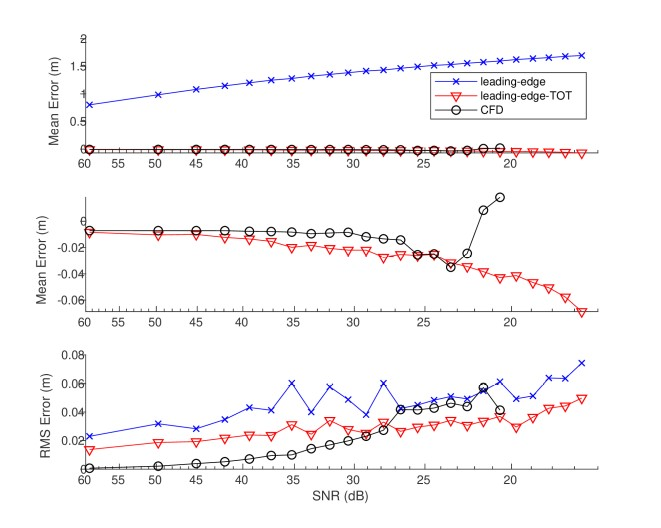
\includegraphics[width=.8\textwidth]{figures/chapter7_TDC/fig_distError_snr.jpg}
\caption{Mean error and RMS error of different timing algorithms}
\label{fig:TDC_Error_beforeFilter}
\end{figure}
The CFD has almost bias at all the distances, while the TOT compensation has increasing negative mean error as distance increases. There are two factors that contribute to the mean error. Note that the TOT compensation calculates the TOF by
\begin{align} \label{eq:TDC_TOT}
TOF=t_{lead}-\Delta_w-t_{start}    
\end{align}
where $t_{lead}$ is the timestamp of the trigger event at the leading edge of a signal, $\Delta_w$ is the walk error obtained from TOT curve, and $t_{start}$ is the arrival time of the transmit signal. The major factor of the negative bias is the inaccurate measurement of $t_{lead}$. As known, the noise on the leading edge of the signal becomes comparative to the pulse at further distance, which causes early triggering of the TDC. An example is given in Figure \ref{fig:TDC_earlyTrigger}, in which the TDC is triggered earlier than it is supposed to be. In that case the $t_{lead}$ is smaller than the ground-truth $t_{lead}$, resulting in a smaller TOF estimation according to Equation \eqref{eq:TDC_TOT}. The statistic measurement of the 500 observations at distance 15m also provides evidence that the measured $t_{lead}$ is 0.15ns (or distance offset of 0.0233m) less than the ground-truth value measured from the noise-free signals. Another factor for the mean error is the inaccurate measurement of the TOT when the SNR is low. Taking the 15m distance for example, the measured TOT from noisy return signals in the experiment is larger than the TOT of the corresponding noise-free signals, which results in that the derived walk error is 0.002m smaller than the ground-truth walk error. However, the inaccurate TOT measurement only contributes slightly to the mean error compared to the early triggering.
\begin{figure}[t!p]
\centering
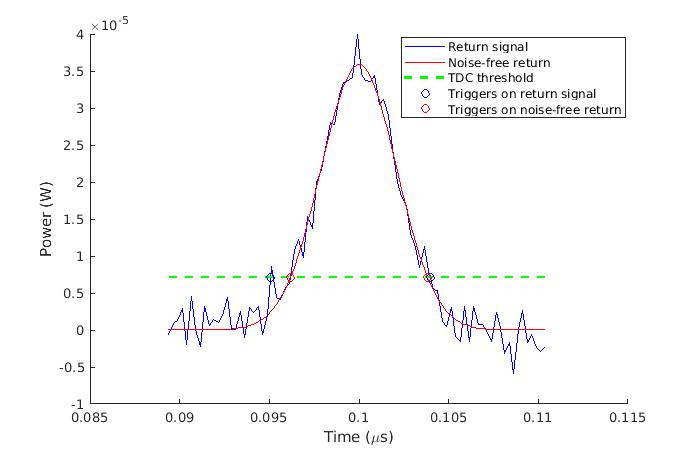
\includegraphics[width=.8\textwidth]{figures/chapter7_TDC/signal_TOT_d_15_trigger.jpg}
\caption{Illustration of early triggering caused by the noise on the leading edge}
\label{fig:TDC_earlyTrigger}
\end{figure}
From the RMS error, we can see all the algorithms are subject to the noise on the signal when the SNR decreases. The traditional leading-edge algorithm is very sensitive to the noise on the signal, while the effect of the noise is compensated to some extent in the TOT algorithm because both the leading edge and falling edge of the signal are taken into account. The CFD algorithm has the least RMS error because the random noise is canceled when the negative attenuated signal is added to the delay signal. However, the CFD method does not work for low SNR conditions (<21.47 dB), because in those cases the amplitude of the attenuated signal is lower than the arming threshold, and the signal is ignored by the algorithm.
\subsection{Low-pass filter}
To reduce the effect of the noise on the TOF estimation, an LP filter with fcut= 0.4GHz was applied to the return signals before the timing algorithms, and the phase shift is compensated. One should note that small orders of the LP should be selected to avoid distortion of the pulse shape. Otherwise, the results of the TOT compensation and the CFD will be affected. The detailed information is given in Section. An example of the filtered signal at a distance of 15 m is given in Figure \ref{fig:TDC_sig_filt}.
\begin{figure}[t!p]
\centering
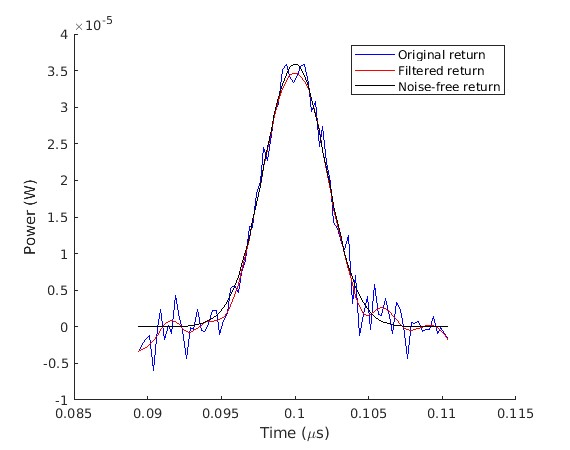
\includegraphics[width=.8\textwidth]{figures/chapter7_TDC/signal_filtered_d15.jpg}
\caption{Original and the filtered signal at a distance of 15m}
\label{fig:TDC_sig_filt}
\end{figure}
\subsection{Results after filtering}
The results after LP filtering are shown in Figure \ref{fig:TDC_Error_afterFilter}. From the Mean error, we can see the positive bias still exists in the traditional leading-edge algorithm because the bias is caused by the walk error which cannot be resolved by the LP filter. On the contrary, the LP filter improves the mean error of the CFD and the TOT compensation. An example of the filtered signal is given in Figure \ref{fig:TDC_earlyTrigger_filt}, in which the noise on the leading edge of the signal is significantly reduced. Statistical results at distance 15m also show the $t_{lead}$ of the filtered noisy signal is only 0.04ns (0.006m distance offset) smaller than the one of noise-free signals, and the difference of walk error is changed to 0.0038m converted to distance. The reduction of the $t_{lead}$ difference also demonstrates the influence of the noise on the TOF measurements. On the other hand, the RMS error of all the algorithms are reduced after the filtering, and the CFD still has the least RMS error followed by the TOT compensation.
\begin{figure}[t!p]
\centering
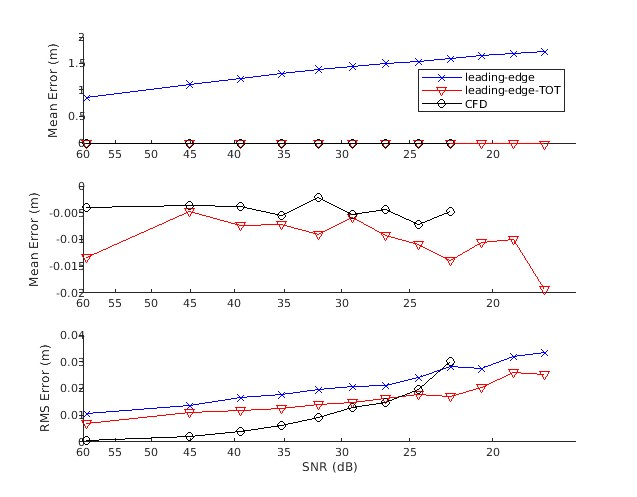
\includegraphics[width=.8\textwidth]{figures/chapter7_TDC/fig_distError_snr_filter.jpg}
\caption{Mean error and RMS error after filtering}
\label{fig:TDC_Error_afterFilter}
\end{figure}

\begin{figure}[t!p]
\centering
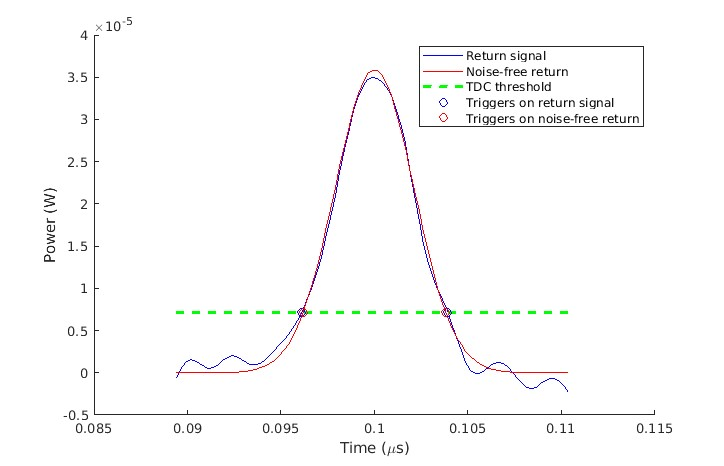
\includegraphics[width=.8\textwidth]{figures/chapter7_TDC/signal_TOT_d_15_trigger_filt.jpg}
\caption{Signal after filtering. Compared to Figure14, the early triggering on the leading edge is significantly reduced by the LP filter}
\label{fig:TDC_earlyTrigger_filt}
\end{figure}